\documentclass{standalone}
\usepackage{tikz}
\usetikzlibrary{patterns, positioning}
\usepackage[sfdefault]{ClearSans} %% option 'sfdefault' activates Clear Sans as the default text font
\usepackage[T1]{fontenc}

\begin{document}
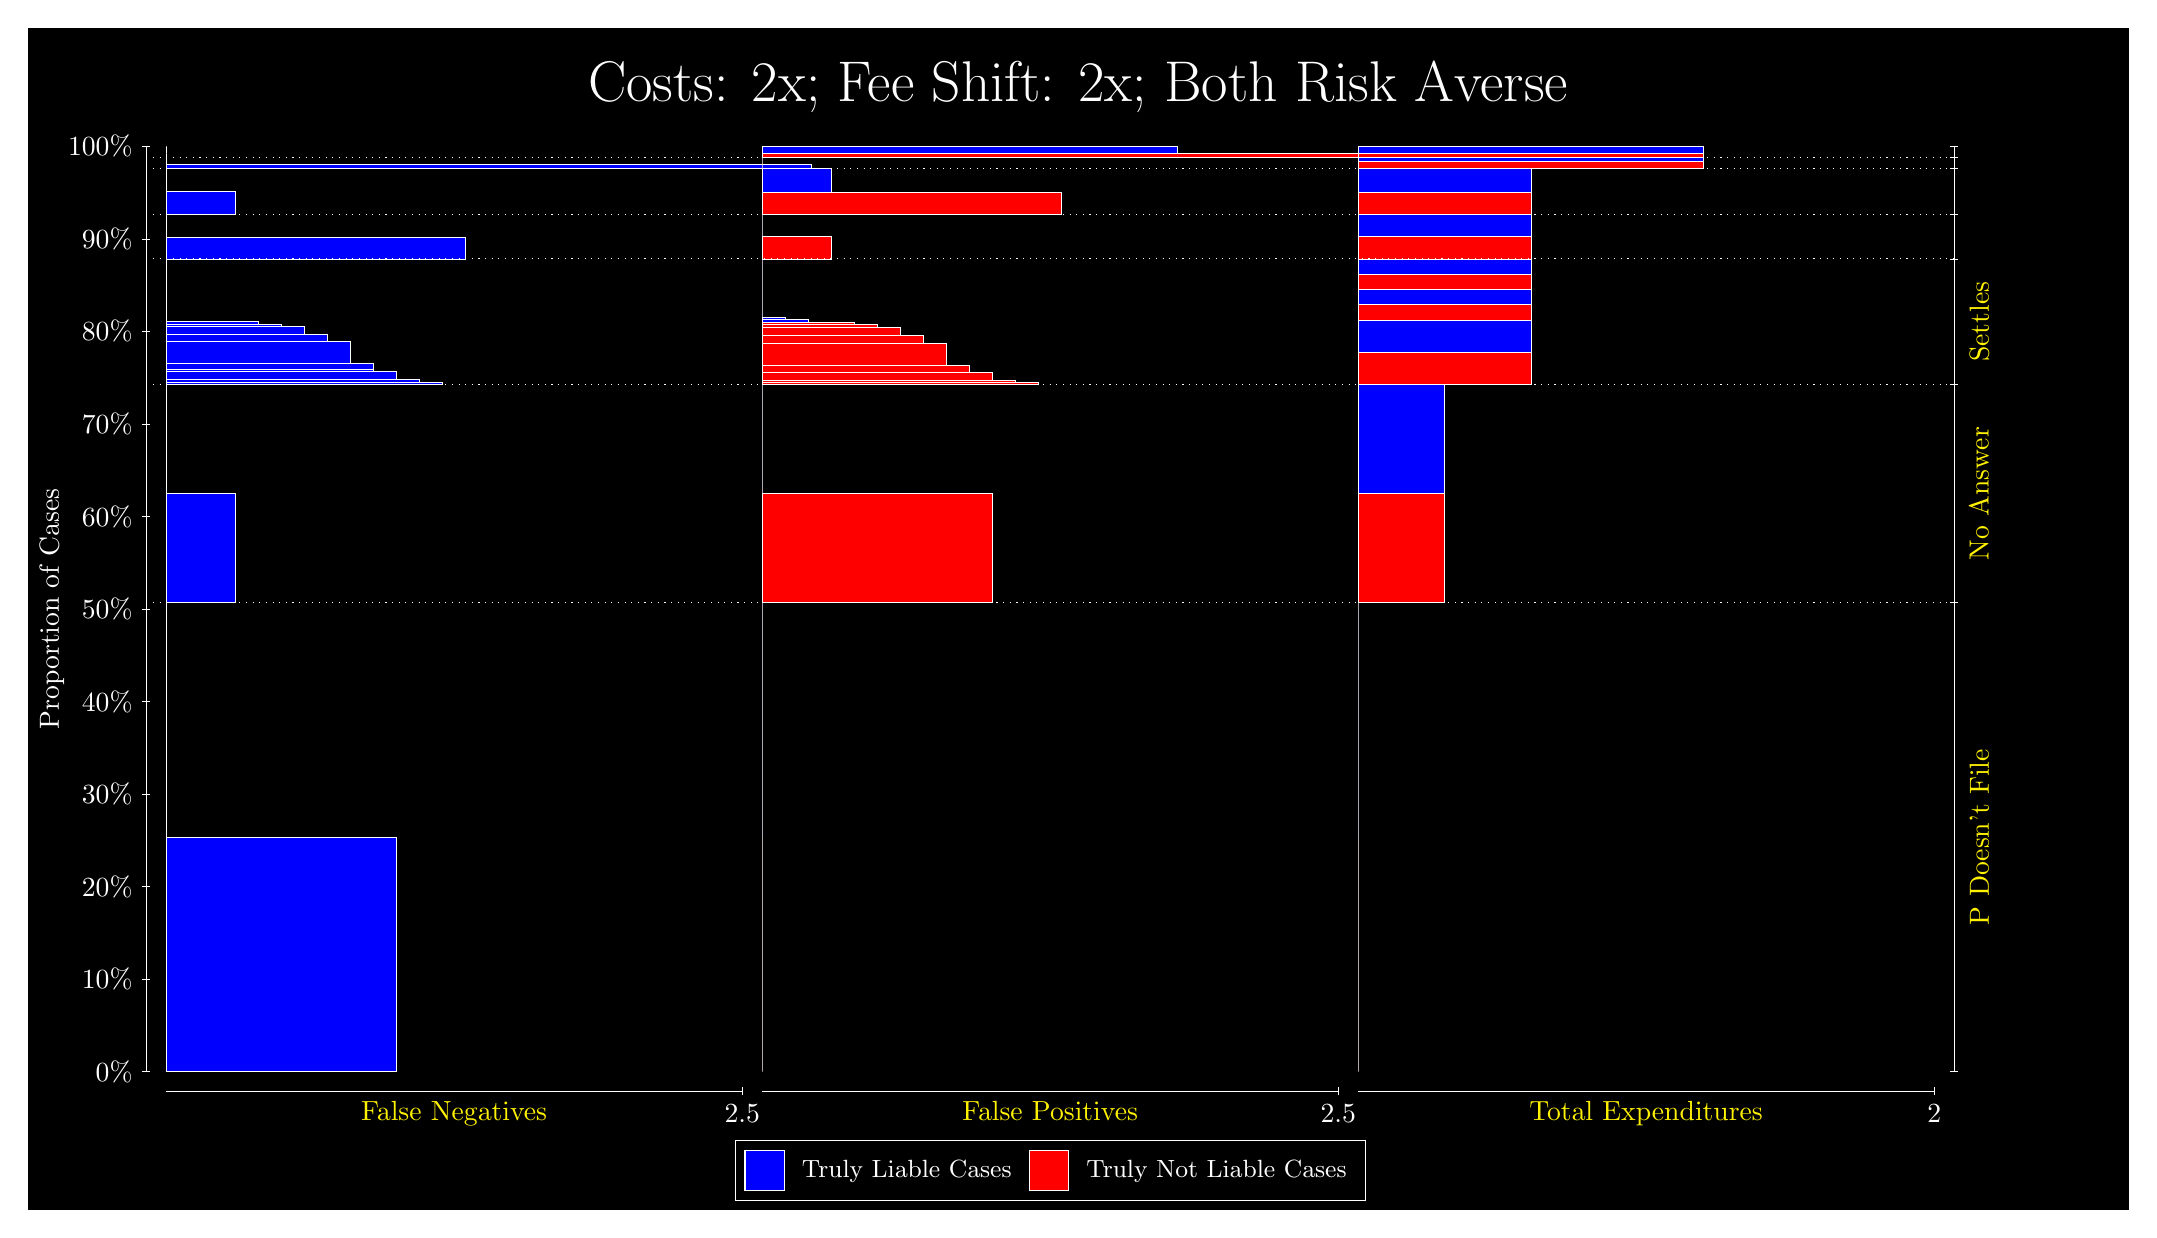
\begin{tikzpicture}
\draw[fill=black] (0,0) rectangle (26.667,15);
\draw[text=white] (0,13.5) rectangle (26.667,15) node[midway] {\huge Costs: 2x; Fee Shift: 2x; Both Risk Averse};
\draw[white, very thin] (1.5,1.75) -- (1.5,13.5);
\node[rotate=90, text=white, anchor=center] at (0.3, 7.625) {Proportion of Cases};
\draw[white, very thin] (1.45,1.75) -- (1.55,1.75);
\node[text=white, anchor=east] at (1.45, 1.75) {0\%};
\draw[white, very thin] (1.45,2.925) -- (1.55,2.925);
\node[text=white, anchor=east] at (1.45, 2.925) {10\%};
\draw[white, very thin] (1.45,4.1) -- (1.55,4.1);
\node[text=white, anchor=east] at (1.45, 4.1) {20\%};
\draw[white, very thin] (1.45,5.275) -- (1.55,5.275);
\node[text=white, anchor=east] at (1.45, 5.275) {30\%};
\draw[white, very thin] (1.45,6.45) -- (1.55,6.45);
\node[text=white, anchor=east] at (1.45, 6.45) {40\%};
\draw[white, very thin] (1.45,7.625) -- (1.55,7.625);
\node[text=white, anchor=east] at (1.45, 7.625) {50\%};
\draw[white, very thin] (1.45,8.8) -- (1.55,8.8);
\node[text=white, anchor=east] at (1.45, 8.8) {60\%};
\draw[white, very thin] (1.45,9.975) -- (1.55,9.975);
\node[text=white, anchor=east] at (1.45, 9.975) {70\%};
\draw[white, very thin] (1.45,11.15) -- (1.55,11.15);
\node[text=white, anchor=east] at (1.45, 11.15) {80\%};
\draw[white, very thin] (1.45,12.325) -- (1.55,12.325);
\node[text=white, anchor=east] at (1.45, 12.325) {90\%};
\draw[white, very thin] (1.45,13.5) -- (1.55,13.5);
\node[text=white, anchor=east] at (1.45, 13.5) {100\%};

\draw[white, very thin] (24.457,1.75) -- (24.457,13.5);
\draw[white, very thin] (24.407,1.75) -- (24.507,1.75);
\node[anchor=west] at (24.407, 1.75) {};
\draw[white, very thin] (24.407,7.7039) -- (24.507,7.7039);
\node[anchor=west] at (24.407, 7.7039) {};
\draw[white, very thin] (24.407,10.474) -- (24.507,10.474);
\node[anchor=west] at (24.407, 10.474) {};
\draw[white, very thin] (24.407,12.07) -- (24.507,12.07);
\node[anchor=west] at (24.407, 12.07) {};
\draw[white, very thin] (24.407,12.634) -- (24.507,12.634);
\node[anchor=west] at (24.407, 12.634) {};
\draw[white, very thin] (24.407,13.215) -- (24.507,13.215);
\node[anchor=west] at (24.407, 13.215) {};
\draw[white, very thin] (24.407,13.357) -- (24.507,13.357);
\node[anchor=west] at (24.407, 13.357) {};
\draw[white, very thin] (24.407,13.5) -- (24.507,13.5);
\node[anchor=west] at (24.407, 13.5) {};

\draw[white, very thin, fill=blue] (1.75,1.75) rectangle (4.6775,4.7269);
\draw[white, very thin, fill=red] (1.75,4.7269) rectangle (1.75,7.7039);
\draw[white, very thin, fill=blue] (1.75,7.7039) rectangle (2.6283,9.0889);
\draw[white, very thin, fill=red] (1.75,9.0889) rectangle (1.75,10.474);
\draw[white, very thin, fill=blue] (1.75,10.474) rectangle (5.2631,10.509);
\draw[white, very thin, fill=blue] (1.75,10.509) rectangle (4.9703,10.54);
\draw[white, very thin, fill=blue] (1.75,10.54) rectangle (4.6775,10.648);
\draw[white, very thin, fill=blue] (1.75,10.648) rectangle (4.3848,10.668);
\draw[white, very thin, fill=blue] (1.75,10.668) rectangle (4.3848,10.745);
\draw[white, very thin, fill=blue] (1.75,10.745) rectangle (4.092,11.028);
\draw[white, very thin, fill=blue] (1.75,11.028) rectangle (3.7993,11.114);
\draw[white, very thin, fill=blue] (1.75,11.114) rectangle (3.5065,11.21);
\draw[white, very thin, fill=blue] (1.75,11.21) rectangle (3.2138,11.241);
\draw[white, very thin, fill=blue] (1.75,11.241) rectangle (2.921,11.273);
\draw[white, very thin, fill=red] (1.75,11.273) rectangle (1.75,12.07);
\draw[white, very thin, fill=blue] (1.75,12.07) rectangle (5.5558,12.342);
\draw[white, very thin, fill=red] (1.75,12.342) rectangle (1.75,12.634);
\draw[white, very thin, fill=blue] (1.75,12.634) rectangle (2.6283,12.933);
\draw[white, very thin, fill=red] (1.75,12.933) rectangle (1.75,13.215);
\draw[white, very thin, fill=blue] (1.75,13.215) rectangle (9.9471,13.266);
\draw[white, very thin, fill=red] (1.75,13.266) rectangle (1.75,13.357);
\draw[white, very thin, fill=red] (1.75,13.357) rectangle (1.75,13.408);
\draw[white, very thin, fill=blue] (1.75,13.408) rectangle (1.75,13.5);
\draw[white, very thin, fill=red] (9.3189,1.75) rectangle (9.3189,4.7269);
\draw[white, very thin, fill=blue] (9.3189,4.7269) rectangle (9.3189,7.7039);
\draw[white, very thin, fill=red] (9.3189,7.7039) rectangle (12.246,9.0889);
\draw[white, very thin, fill=blue] (9.3189,9.0889) rectangle (9.3189,10.474);
\draw[white, very thin, fill=red] (9.3189,10.474) rectangle (12.832,10.505);
\draw[white, very thin, fill=red] (9.3189,10.505) rectangle (12.539,10.535);
\draw[white, very thin, fill=red] (9.3189,10.535) rectangle (12.246,10.633);
\draw[white, very thin, fill=red] (9.3189,10.633) rectangle (11.954,10.723);
\draw[white, very thin, fill=red] (9.3189,10.723) rectangle (11.661,11.004);
\draw[white, very thin, fill=red] (9.3189,11.004) rectangle (11.368,11.097);
\draw[white, very thin, fill=red] (9.3189,11.097) rectangle (11.075,11.202);
\draw[white, very thin, fill=red] (9.3189,11.202) rectangle (10.783,11.236);
\draw[white, very thin, fill=red] (9.3189,11.236) rectangle (10.49,11.271);
\draw[white, very thin, fill=blue] (9.3189,11.271) rectangle (9.9044,11.303);
\draw[white, very thin, fill=blue] (9.3189,11.303) rectangle (9.6116,11.334);
\draw[white, very thin, fill=blue] (9.3189,11.334) rectangle (9.3189,12.07);
\draw[white, very thin, fill=red] (9.3189,12.07) rectangle (10.197,12.362);
\draw[white, very thin, fill=blue] (9.3189,12.362) rectangle (9.3189,12.634);
\draw[white, very thin, fill=red] (9.3189,12.634) rectangle (13.125,12.916);
\draw[white, very thin, fill=blue] (9.3189,12.916) rectangle (10.197,13.215);
\draw[white, very thin, fill=red] (9.3189,13.215) rectangle (9.3189,13.306);
\draw[white, very thin, fill=blue] (9.3189,13.306) rectangle (9.3189,13.357);
\draw[white, very thin, fill=red] (9.3189,13.357) rectangle (17.516,13.408);
\draw[white, very thin, fill=blue] (9.3189,13.408) rectangle (14.588,13.5);
\draw[white, very thin, fill=red] (16.888,1.75) rectangle (16.888,4.7269);
\draw[white, very thin, fill=blue] (16.888,4.7269) rectangle (16.888,7.7039);
\draw[white, very thin, fill=red] (16.888,7.7039) rectangle (17.986,9.0889);
\draw[white, very thin, fill=blue] (16.888,9.0889) rectangle (17.986,10.474);
\draw[white, very thin, fill=red] (16.888,10.474) rectangle (19.083,10.883);
\draw[white, very thin, fill=blue] (16.888,10.883) rectangle (19.083,11.294);
\draw[white, very thin, fill=red] (16.888,11.294) rectangle (19.083,11.488);
\draw[white, very thin, fill=blue] (16.888,11.488) rectangle (19.083,11.682);
\draw[white, very thin, fill=red] (16.888,11.682) rectangle (19.083,11.876);
\draw[white, very thin, fill=blue] (16.888,11.876) rectangle (19.083,12.07);
\draw[white, very thin, fill=red] (16.888,12.07) rectangle (19.083,12.362);
\draw[white, very thin, fill=blue] (16.888,12.362) rectangle (19.083,12.634);
\draw[white, very thin, fill=red] (16.888,12.634) rectangle (19.083,12.916);
\draw[white, very thin, fill=blue] (16.888,12.916) rectangle (19.083,13.215);
\draw[white, very thin, fill=red] (16.888,13.215) rectangle (21.279,13.306);
\draw[white, very thin, fill=blue] (16.888,13.306) rectangle (21.279,13.357);
\draw[white, very thin, fill=red] (16.888,13.357) rectangle (21.279,13.408);
\draw[white, very thin, fill=blue] (16.888,13.408) rectangle (21.279,13.5);
\draw[white, dotted] (1.5,7.7039) -- (24.457,7.7039);
\draw[white, dotted] (1.5,10.474) -- (24.457,10.474);
\draw[white, dotted] (1.5,12.07) -- (24.457,12.07);
\draw[white, dotted] (1.5,12.634) -- (24.457,12.634);
\draw[white, dotted] (1.5,13.215) -- (24.457,13.215);
\draw[white, dotted] (1.5,13.357) -- (24.457,13.357);
\draw[white, very thin] (1.75,1.5) -- (9.0689,1.5);
\node[text=yellow, anchor=north] at (5.4094, 1.5) {False Negatives};
\draw[white, very thin] (9.0689,1.45) -- (9.0689,1.55);
\node[text=white, anchor=north] at (9.0689, 1.45) {2.5};

\draw[white, very thin] (9.3189,1.5) -- (16.638,1.5);
\node[text=yellow, anchor=north] at (12.978, 1.5) {False Positives};
\draw[white, very thin] (16.638,1.45) -- (16.638,1.55);
\node[text=white, anchor=north] at (16.638, 1.45) {2.5};

\draw[white, very thin] (16.888,1.5) -- (24.207,1.5);
\node[text=yellow, anchor=north] at (20.547, 1.5) {Total Expenditures};
\draw[white, very thin] (24.207,1.45) -- (24.207,1.55);
\node[text=white, anchor=north] at (24.207, 1.45) {2};

\node[text=yellow, centered, rotate=90] at (24.777, 4.7269) {P Doesn't File};
\node[text=yellow, centered, rotate=90] at (24.777, 9.0889) {No Answer};
\node[text=yellow, centered, rotate=90] at (24.777, 11.272) {Settles};





\draw (12.978300999999998,1.5) node[draw=none] (baseCoordinate) {};
\begin{scope}[align=center]
        \matrix[scale=0.5, draw=white, below=0.5cm of baseCoordinate, nodes={draw}, column sep=0.1cm]{
            \node[rectangle, draw, minimum width=0.5cm, minimum height=0.5cm, fill=blue] {}; &
            \node[draw=none, font=\small, text=white] (B) {Truly Liable Cases}; &
            \node[rectangle, draw, minimum width=0.5cm, minimum height=0.5cm, fill=red] {}; &
            \node[draw=none, font=\small, text=white] (B) {Truly Not Liable Cases}; \\
            };
\end{scope}

\end{tikzpicture}
\end{document}